\begin{frame}[allowframebreaks,allowdisplaybreaks]
    \subsection{Definition}
    \frametitle{B-Tree Definition}
    \begin{columns}
        \begin{column}{\textlecolumn}
            \begin{block}{}
                \begin{itemize}
                    \item We will define that \(T\), an object, is a B-Tree if they are an instance of the class.
                    \[
                        T \in t\left(\alpha, h\right)
                    \]
                    \item Where \(h\) is the height of the B-Tree.
                    \item And, \(\alpha\) is a predefined constant.
                    \item This type of balanced tree have a higher degree than the previous trees.
                    \item Or in simple words, they have more than 1 key and 2 sub-trees in each node.
                    \item Keep in mind that in B-Trees, \textbf{leafs are not nodes}.
                    \item This higher degree have a cuple of properties added to it, which we need to check and prove
                    \item Also, due to the higher degree of the nodes, we will have to change the 
                        \lstinline|find|, \lstinline|insert| and \lstinline|delete| operations of the B-Tree.
                \end{itemize}
            \end{block}
        \end{column}
        \begin{column}{\textricolumn}
        \end{column}
    \end{columns}
    
    \framebreak{}
    \begin{columns}
        \begin{column}{0.35\textwidth}
                \begin{figure}
                    \includegraphics[%
                        width=\textwidth,%
                        page=2,%
                        ]{resources/made/B-Trees_general.pdf}
                    \caption[]{Node of a B-Tree}
                \end{figure}
        \end{column}
        \begin{column}{0.35\textwidth}
                \begin{figure}
                    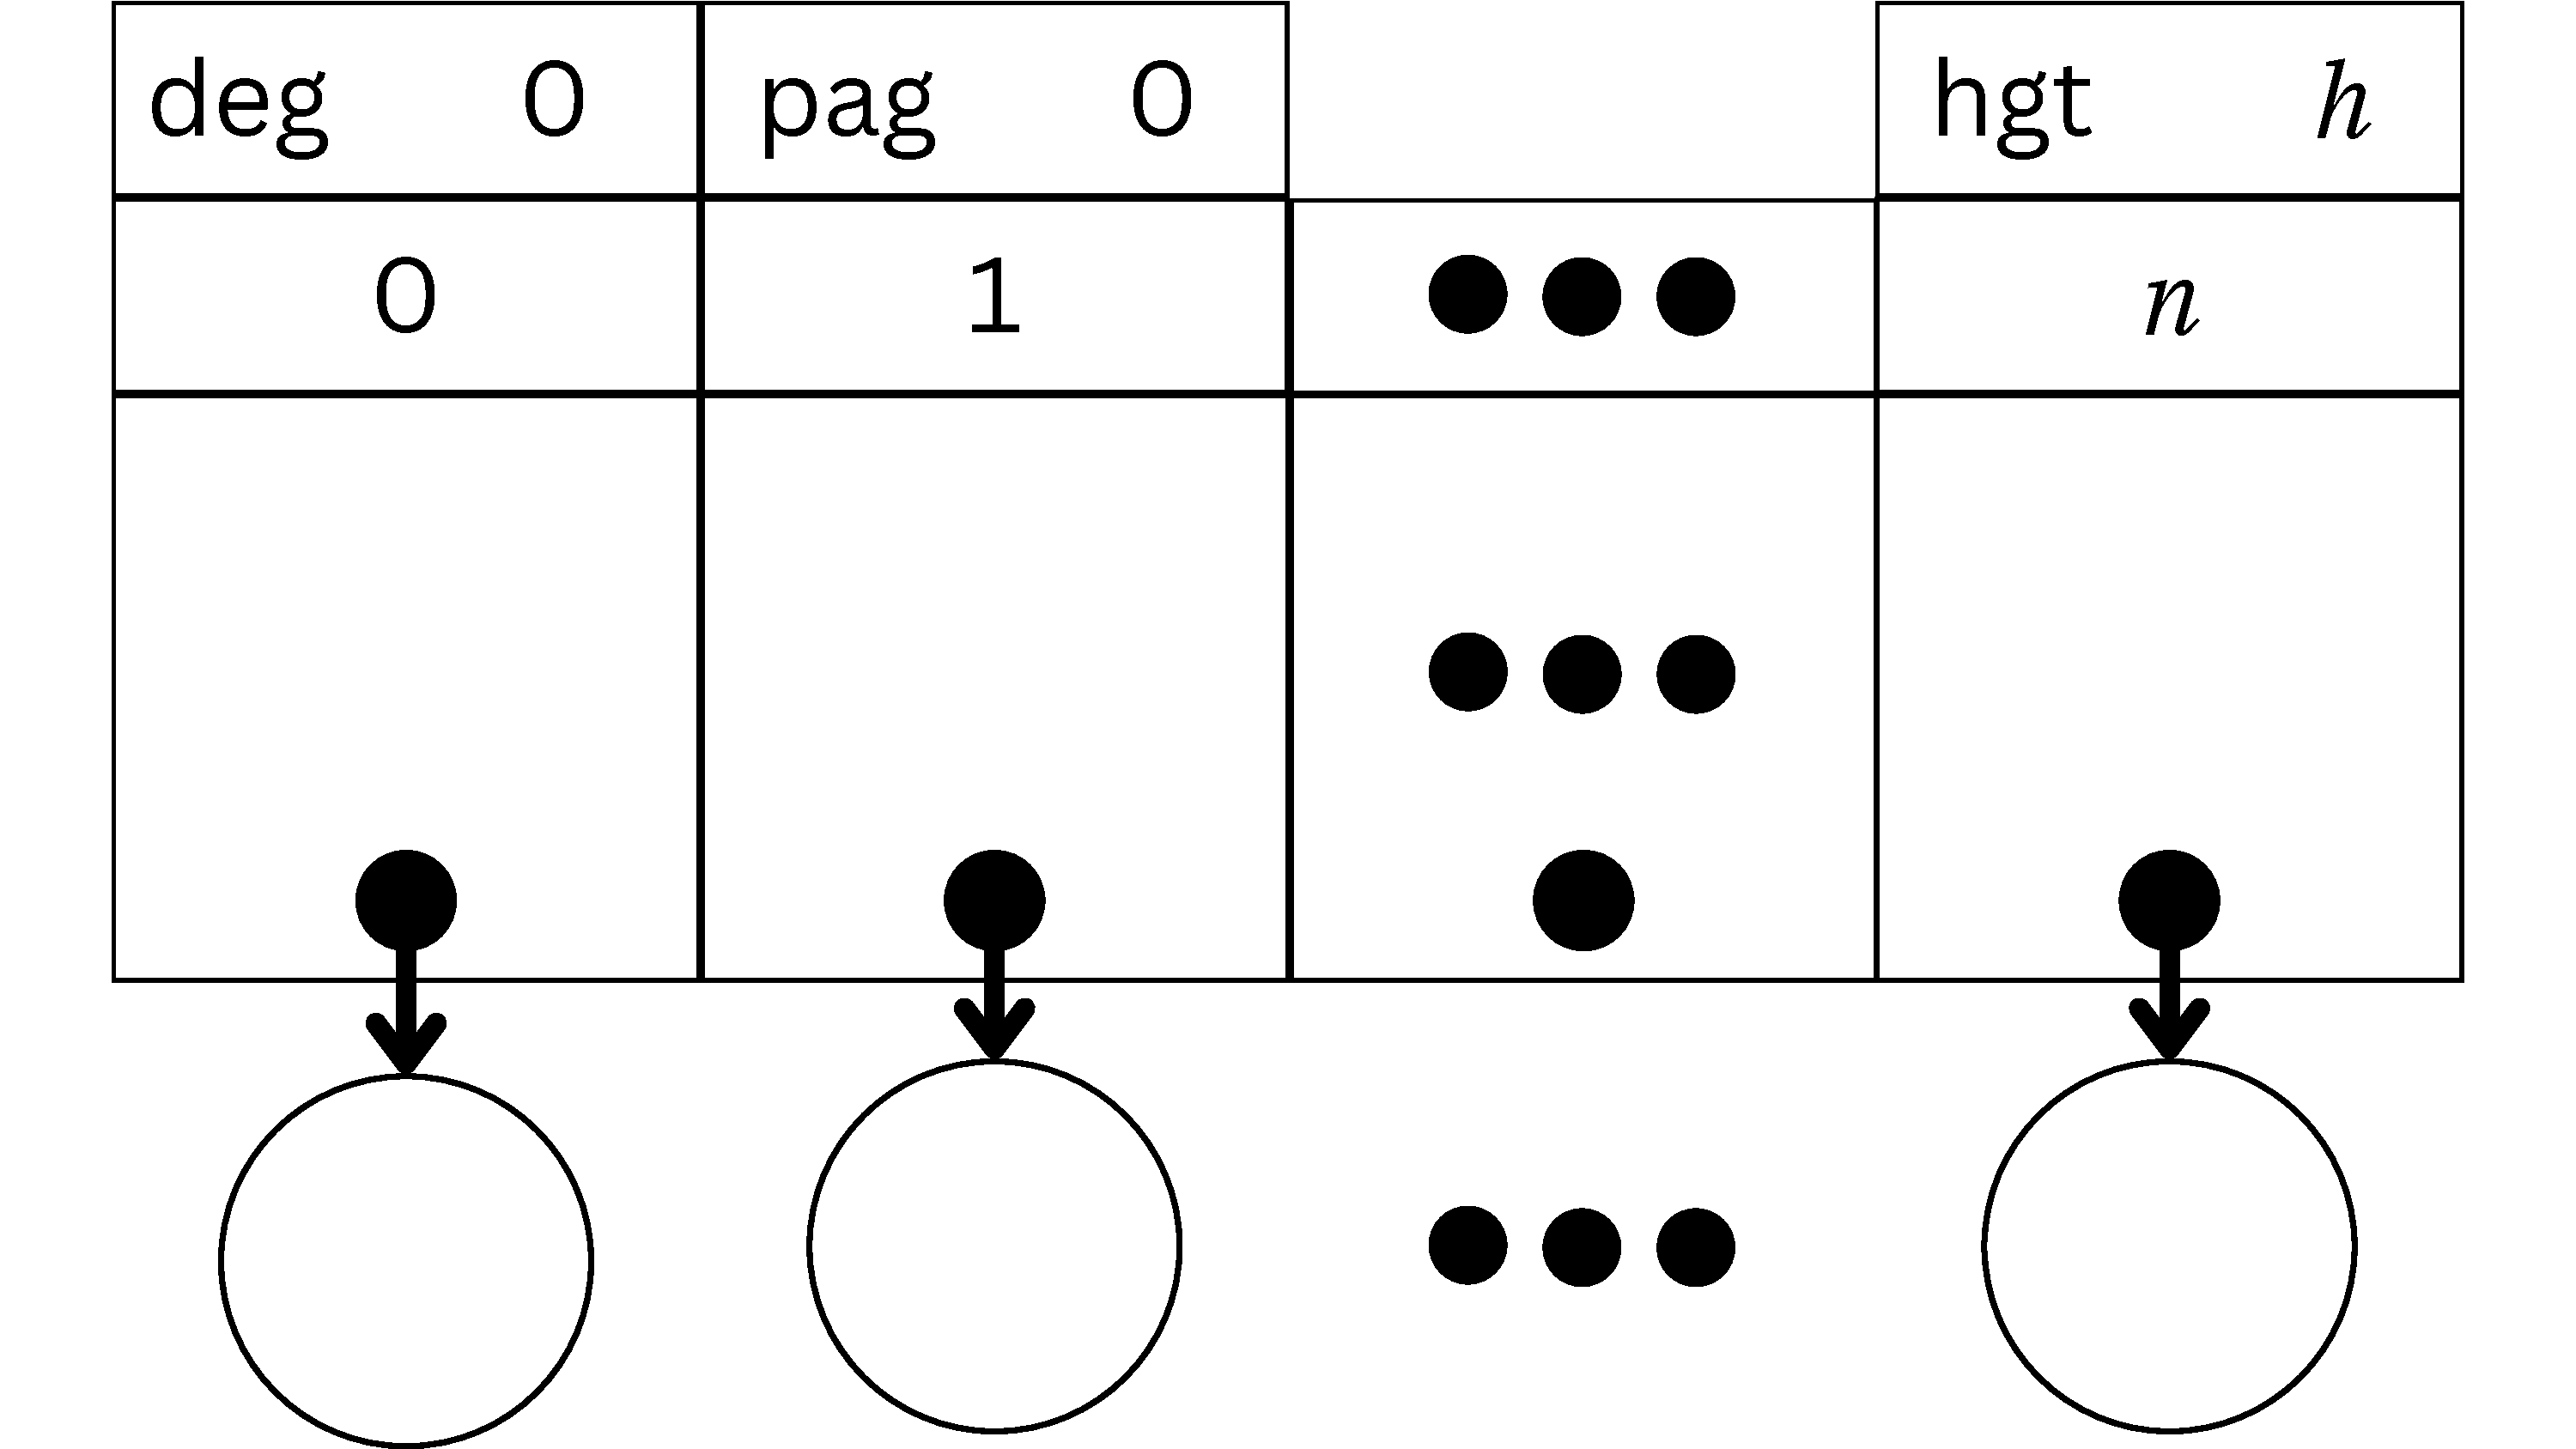
\includegraphics[%
                        width=\textwidth,%
                        page=1,%
                        ]{resources/made/B-Trees_general.pdf}
                    \caption[]{Leaf of a B-Tree}
                \end{figure}
        \end{column}
    \end{columns}
    \begin{figure}
        \includegraphics[%
            width=0.35\textwidth,%
            page=3,%
            ]{resources/made/B-Trees_general.pdf}
        \caption[]{Generic Node of a B-Tree}
    \end{figure}
\end{frame}
